\chapter{Upgrade on the ATLAS Calorimeter Trigger}
\chapterquote{To infinity … and beyond!}{Buzz Lightyear (made in Taiwan), Toy Story}
Following the period of LHC operation with $\sqrt{s}=13$ from 2015 to 2018, we are now in the long-shutdown period (LS2) in preparation for the Run~3 operation which will start in 2021. The major upgrades in this period are to enhance the LHC energy for proton-proton collision as well the luminosity. Meanwhile, three main upgrades will be also performed on the ATLAS detector: the new small wheel (NSW) in the muon spectrometer\cite{STELZER20161160}, the fast tracking trigger at HLT\cite{Shochet:1552953}, and the new L1Calo infrastructure. One of the main purposes of the two upgrades is to improve the trigger rate for better recognition on the physical objects. This chapter will be dedicated to the L1Calo Run~3 upgrade from the hardware design, preparation of the software, to expected performance of the new L1Calo infrastructure, for which I was in charge of the software preparation and also the $E^{miss}_{T}$ trigger algorithm. 
\section{LHC Run~3 Upgrade}
After the operation of Run~2 (2015-2018), the LHC is now undergoing the Long Shutdown period (LS2) during which a couple of upgrades and maintenance will be taken to enhance the LHC performance to prepare for the upcoming operation in 2021. This is to bring the LHC to the design energy of $7~TeV$ for each beam and also enhance the instantaneous luminosity to $2\times10^{34}~cm^{-2}s^{-1}$ with estimated $\sim 70$ pile-ups per bunch crossing which doubles the nominal LHC luminosity. This operation is expected to last for three years delivering the integrated data of $300~fb^{-1}$ by the end of this period. This upgrade plan could also be taken as the preceding work for the High-Luminosity LHC (HL-LHC) which will keep the beams at $7~TeV$, but the instantaneous luminosity will increase to $7.5\times10^{34}~cm^{-2}s^{-1}$ for which the pile-ups will go up to 200 per bunch crossing. The LHC upgrade road map and the estimated instantaneous luminosity could be seen in Fig.~\ref{Fig:LHC_upgrade}.
\begin{figure}[!h]                
	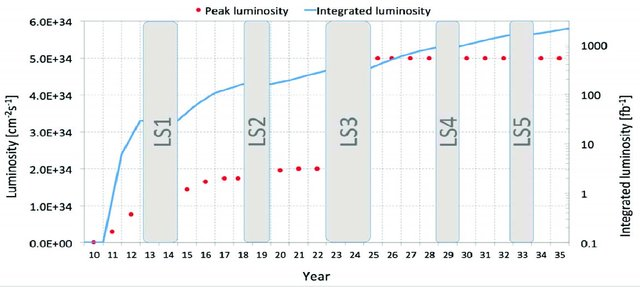
\includegraphics[width=0.9\textwidth]{Chapter6/The-LHC-upgrade-schedule-and-associated-luminosity.jpg}
	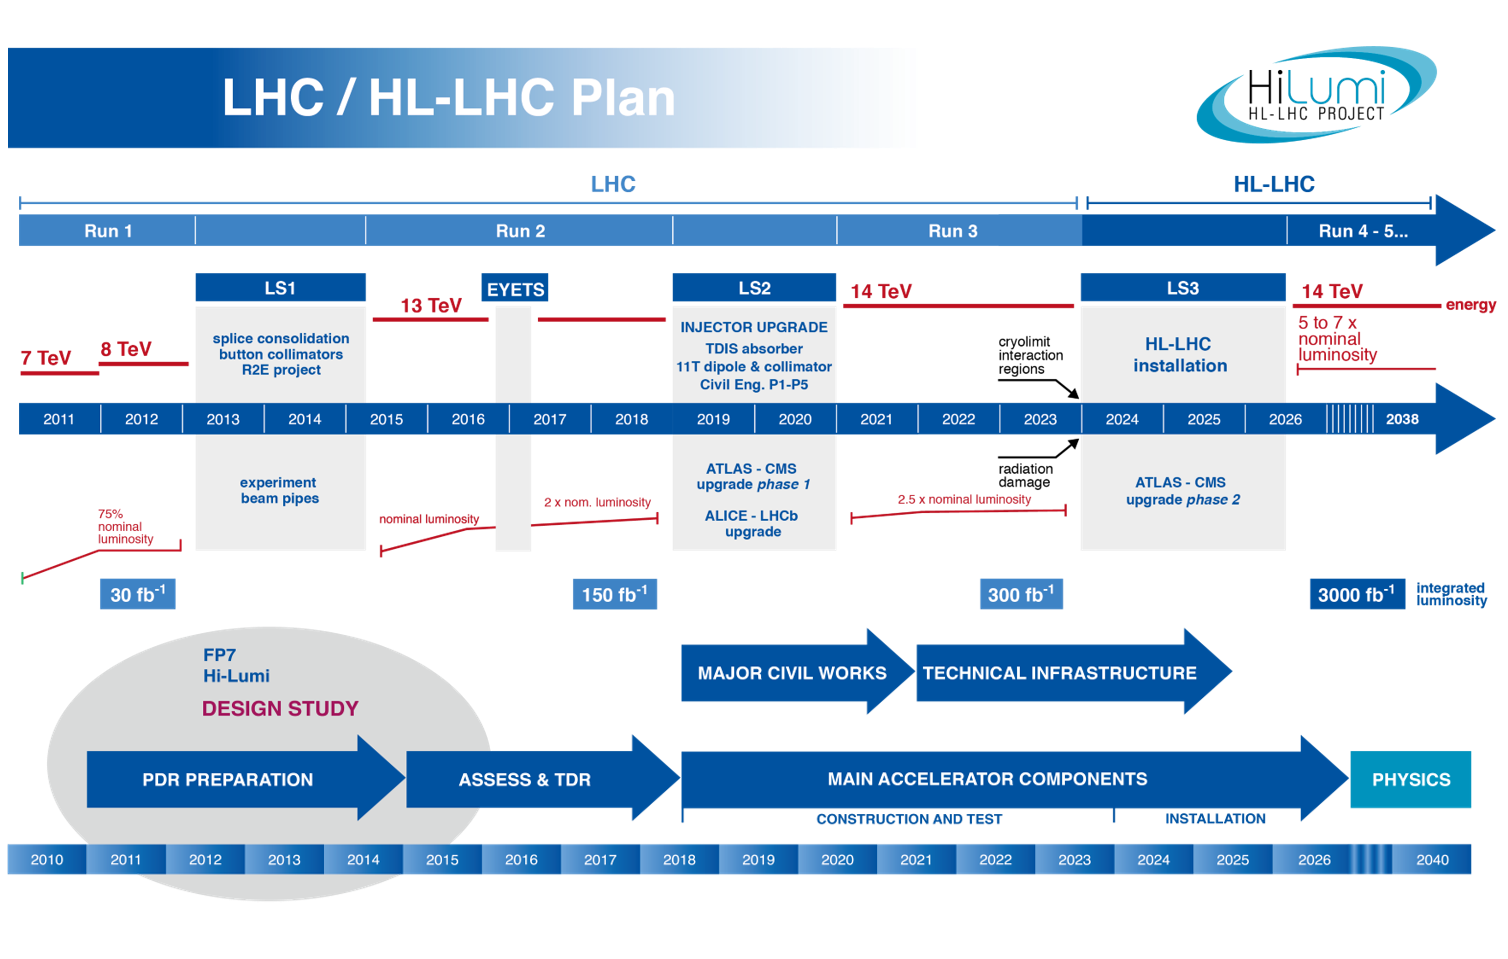
\includegraphics[width=0.95\textwidth]{Chapter6/Schedule_HL.png}
	\begin{center}
		\caption{The LHC upgrade plan (top)\cite{schedule} and the instantaneous luminosity (bottom)\cite{Atlas:2019qfx} for the upcoming 10 years with the estimated integrated data.}
		\label{Fig:LHC_upgrade}            
	\end{center}
\end{figure} 
\noindent
\\
\\The major upgrade of this project is that the injector of beams will be replaced by the new LINAC4, and the LINAC2 will just retire from 40~years of operation. The major difference between the LINAC2 and LINAC4 is that the LINAC4 will accelerate negatively charged hydrogen ions ($H^{-1}$), and the electrons will be stripped off in the PSB, which design is intended to concentrate the beams with better stability\cite{LINAC4}. Furthermore, the CERN acceleration complex (Fig.~\ref{Fig:boost}) will also upgrade the RF cavities for the energy upgrade. For the LHC itself, the upgrade will take place in the magnet systems for which more than 20 magnets will be replaced, and the new superconductor technology will also be employed with the new magnet material which can afford the even higher magnetic field of $\sim 10~T$ (the original material can only take the magnetic field up to $\sim 9~T$)\cite{LINAC4}. 
\\
\\This upgrade project is aiming to refine the present physics results. Firstly, the Higgs boson properties like the couplings to other particles or themselves could be measured with better precision to verify the SM predictions. Secondly, most of the SM interactions have the cross-sections as a function of the collision centre-of-mass energy, and the new operation energy could provide other measurement points. Thirdly, the increase of collected data will benefit the new physics search giving a better separation on the test statistics between hypotheses, and this will enhance the sensitivity to the hidden particles. \cite{Atlas:2019qfx} has summarized all the studies for expected results with the Run~3 LHC data.
\section{Hardware of the Run~3 ATLAS Calorimeter Trigger}
To incorporate the upcoming LHC upgrades, the ATLAS hardware calorimeter trigger system is scheduled to undergo a series of upgrade to cope with the unprecedented luminosity in Run~3, and it will also be remained as part of the Run~4 L0 trigger. The full L1Calo trigger scheme in Run~3 can be seen in Fig.~\ref{Fig:l1calo_scheme}.
\begin{figure}[!h]                
	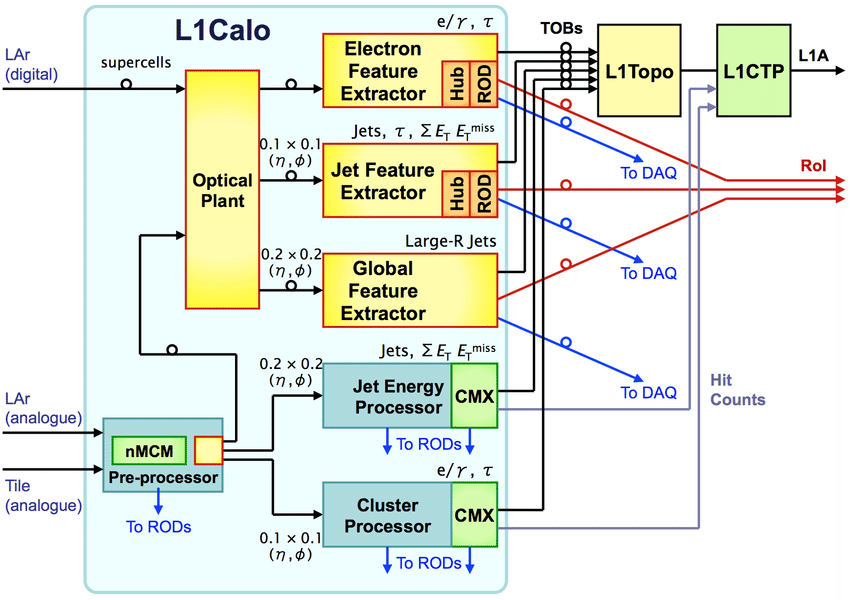
\includegraphics[width=0.93\textwidth]{Chapter6/L1Calo.png}
	\begin{center}
		\caption{The L1Calo hardware scheme in the Run~3 operation\cite{Schwienhorst:2016efd}}
		\label{Fig:l1calo_scheme}            
	\end{center}
\end{figure}
\noindent
It could be noted that the Run~2 system will still remain in the operation for the tile calorimeter input running in parallel with the new system and also for the purpose of commissioning. This design is due to the reason that the calorimeter readout upgrade will only take place in the LAr detector for which the output signal will be digitized, and the tile detector would still use the legacy analogue system. The newly digitized signal from the LAr detector will be processed into the trigger-level object, ``supercells'' (a new type of trigger tower), in the ``LAr Digital Processing Blade'' (LDPB) with a granularity of $0.025\times0.1$ for the middle layer and sent to the optical plant once per 25~ns (the LHC collision rate). Before the transmission into the object processors, two others new types of trigger towers will be constructed from supercells as well in LDPB, jTowers and gTowers, within the Data Processing System (DPS) which is part of the LDPB. The calorimeter information is herein duplicated into these three types of trigger towers, and they are distributed by the optical plant to the three feature extractors respectively: supercells to the electron feature extractor (eFex), jTowers to the jet feature extractor (jFex), and gTowers to the global feature extractor (gFex). Those Fex systems are designed as FPGA boards written in the reconstruction algorithms which will then output the physical objects to the L1Topo and L1CTP to make the trigger decision along with the outputs from L1MU. Regarding of the tile detector, the analogue signal is processed by a new processor, ``Tile Rear Extension Module'' (TREX), into ``tTowers'' with the granularity of $0.1\times0.1$, and they will be taken into the Fex's as well. In comparison to the Run~2 trigger system, the reconstruction of physical objects could access a better granularity for the background suppression and also have a longer latency for more complicated algorithms of physical object reconstruction.   
\\
\\{\bf eFex and Supercells}
\\
\\The eFex is designed to reconstruct the electromagnetic objects like electrons, photons, and taus, with the trigger towers of best granularity, supercells. With respect to the other two trigger tower types (jTowers and gTowers), supercells are constructed within each layer in the LAr calorimeter, and the layer names in each detector region from inside to outside are:
\begin{itemize}
	\item Barrel ($0<|\eta|<1.52$): PreSamplerB, EMB1, EMB2, EMB3 \\ (EMB stands for ``EM Barrel'')
	\item Barrel ($1.52<|\eta|<3.2$): PreSamplerE, EME1, EME2, EME3, HEC \\ (EME stands for ``EM Endcap'', and HEC stands for Hadronic Endcap)
	\item Barrel ($3.2<|\eta|$): FCAL1, FCAL2, FCAL3
\end{itemize}
Although the hadronic endcap calorimeter still has several layers, the system would still just sum their energy deposit as one entity. Due to the detector structure, some of the layers might not have the full extent within the designated region. In terms of the granularity, the middle two layers (EMB1 and EMB2) have the finest one with $0.025\times 0.1$ in the $\Delta\eta\times\Delta\phi$ plane, while it is $0.1\times0.1$ for the front and back layers (Presampler and EMB3) in the barrel region. However, this supercell arrangement is not employed in the full LAr detector, and the granularity gets more coarse when $|\eta|$ increases. In the forward region, the most coarse granularity would degrade to $0.32\times0.4$ for the back layer of the forward detector (this is a rough number, as the forward supercells are in irregular shapes due to the complicated structure geometry in this region). The comparison between supercells and Run2 trigger towers could be seen in Fig.~\ref{Fig:tt_compar}. Different from the Run~2 trigger towers, the layer information will be kept in Run~3 L1Calo system, and the middle two layers of supercells have finer granularity. This indicates the accessibility to isolation variables with more complicated algorithm. The full detail of the granularity and the coverage of each layer could be found in \cite{Aleksa:1602230}. This is the key upgrade for the new L1Calo system. In the Run~2 operation, the single electron trigger has taken around $30\%$ of the total output bandwidth, and this limits the bandwidth budget for the other signatures like jets or taus. Therefore, the eFex upgrade is aiming to make better suppression on the background and keeping the same efficiency for physical signal like $Z\to ee$. 
\begin{figure}[!h]                
	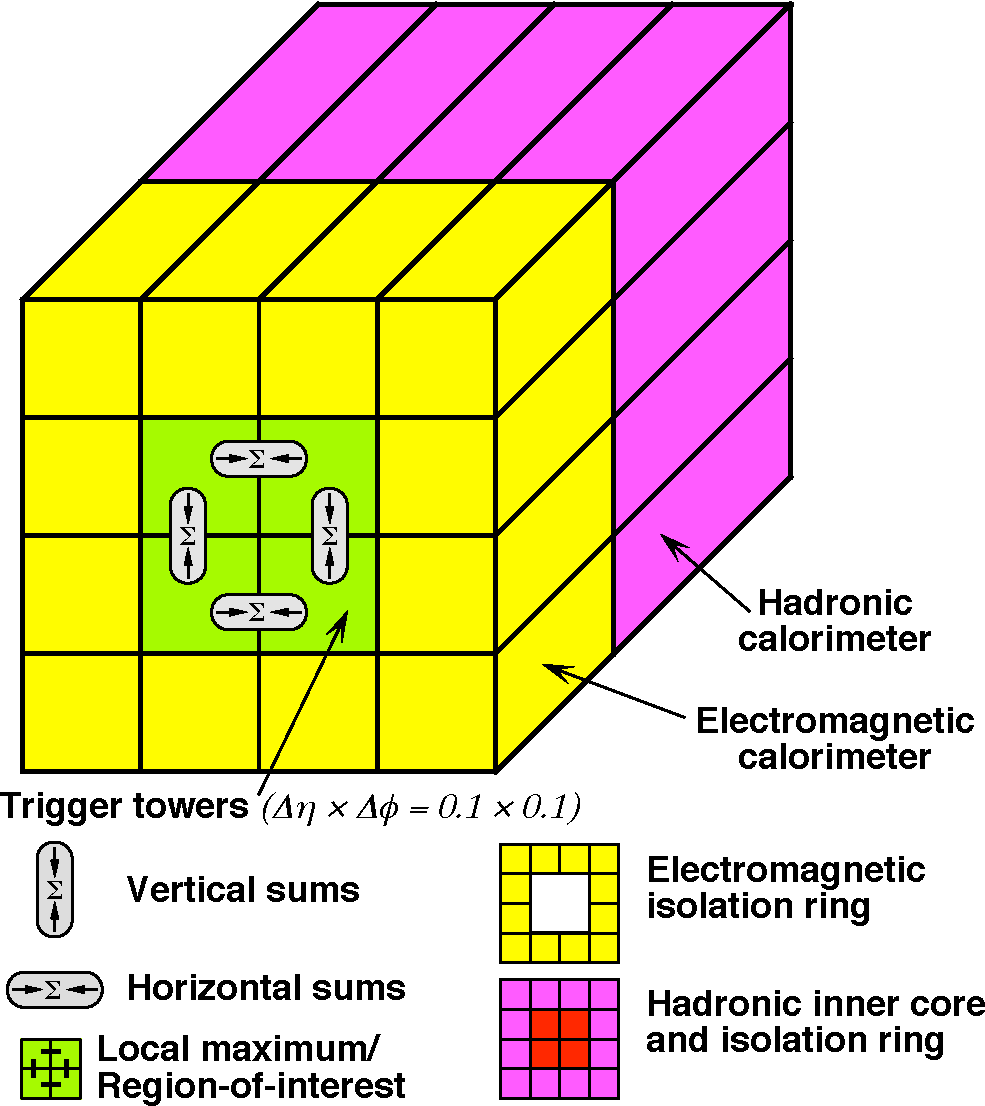
\includegraphics[width=0.35\textwidth]{Chapter6/Run2TT.pdf}
	\includegraphics[width=0.62\textwidth]{Chapter6/Supercell.png}
	\begin{center}
		\caption{The comparison of the Run~2 trigger towers\cite{Aleksa:1602230} and the supercells\cite{Aaboud:2016leb} in the barrel region. One block in the Run~2 trigger tower is corresponding to one square in the front layer of supercells. }
		\label{Fig:tt_compar}            
	\end{center}
\end{figure}
\noindent
\\
\\To evaluated the energy of each supercell, the signal of cells is sent to a processor called ``LATOME'' with an optimal filter (OF). The received analogue LAr cell signal is firstly digitalized through the analogue digital converter (ADC) into the number of ADC counts. The energy is then calibrated by the optimal filter to estimated the measured transverse energy ($E_{T}=E\times\cos\theta$) and also mitigate the noise:
\begin{equation}
\label{Eq:get_Et}
E_{T}=\displaystyle\sum_{i=1}^{i=4}\alpha_{i}S_{i}
\end{equation}
\begin{equation}
\label{Eq:get_tau}
E_{T}\cdot\tau=\displaystyle\sum_{i=1}^{i=4}\beta_{i}S_{i}
\end{equation}
\noindent
S is taken as the ADC count with the optimal filter coefficients (OFC), $\alpha$ and $\beta$, and $\tau$ is the phase shift along the measured time to ensure the energy is assigned to the appropriate bunch crossing. The i is the index for energy sampling every 25~ns within an active window of 100~ns. It should be noted that although the collision rate of LHC is one bunch crossing per 25~ns, the active window for ``one'' collision is still 100~ns. This means once a channel receives the signal, it will not be available for the following few bunch crossings. In Run~2, the timing assignment was simply applied by checking whether a peak of pulse could be found within the active window\cite{Jongmanns:2661780} (peak finder algorithm):
\begin{equation}
S_{i-1}<S_{i}>S_{i+1}\quad 
\end{equation}
However, for the search of long-lived particles, they might arrive in the calorimeter after this time window. Therefore, a more flexible algorithm to extend the time window will be implemented in the Run~3,
\begin{equation}
\begin{cases}
-8~ns<t<16~ns & E_{T}\geq 10~GeV \\
-8~ns<t<8~ns & E_{T}<10~GeV \\
\end{cases}
\end{equation}
Under this case, the new $E_{T}$ measured from Eq.~\ref{Eq:get_tau} is to recover the peak after it is shifted by the OF. Although the sampling period is 25~ns, the sampling window could be delayed by maximally 24~ns with the steps of 1~ns using the PHOS4 chip\cite{Toifl:1999qv}, which can help to achieve the desired temporal resolution. Fig.~\ref{Fig:OFC} is presenting how the OFC shifts the peak of the origin digitalized ADC input from the beam test and the supercell energy efficiency after the new timing cuts from simulation. They are showing that the new algorithms could successfully recover the peak energy and also reach the signal plateau of 3~GeV energy deposit in a supercell.
\begin{figure}[!h]                
	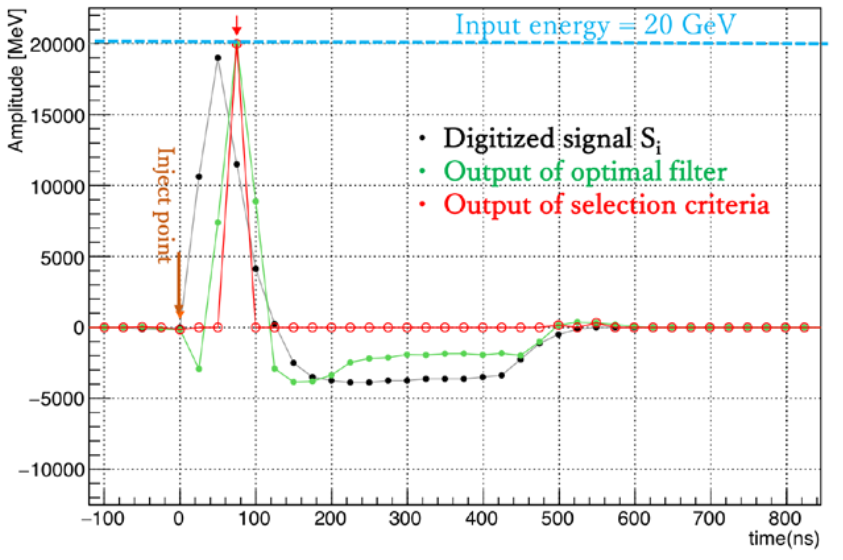
\includegraphics[width=0.48\textwidth]{Chapter6/Pulse.png}
	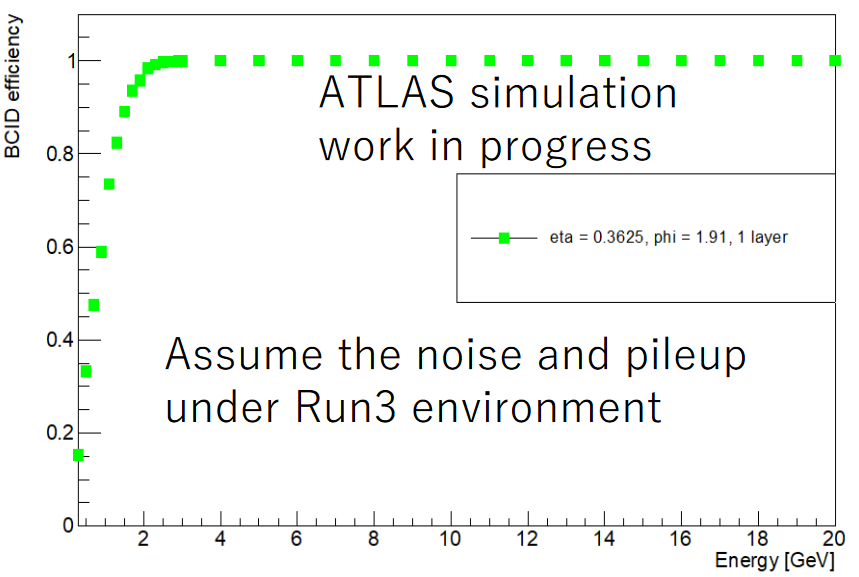
\includegraphics[width=0.48\textwidth]{Chapter6/TimeWindow.png}
	\begin{center}
		\caption{The digitized pulse shape from the ADC and the signal efficiency after the timing window cut. The peak could be seen shifted after the OF is applied, and the timing window properly removes the negative measured energy. }
		\label{Fig:OFC}            
	\end{center}
\end{figure}
\noindent
\\
\\The other correction on the supercells is the ``pedestal correction''. When the LAr cells start to receive the energy from a bunch train, the cell would deliver strong noise during the first few bunches ($\sim 20$ bunches), and it leads to a high trigger rate beyond the trigger rate budget. The pedestal correction is applied to mitigate the effect by reducing the energy count from the ADC. Fig.~\ref{Fig:pc} is showing the pedestal correction used in the Run~2 operation, while its optimization for Run~3 is still ongoing. Therefore, in the following studies, the first 20 bunches of a bunch train are vetoed in the event selection to remove this noise source. The average noise response (the energy deposit from $pp\to jj$ for which the two jets are with $E_{T}<20~GeV$ at truth level) for each layer in the Run~3 simulated environment ($\mu\sim80$) could be seen Fig.~\ref{Fig:sc_noise}, and the noise would increase with $|\eta|$ due to the fact that the supercells are larger in the high $|\eta|$ region.
\begin{figure}[!h]                
  	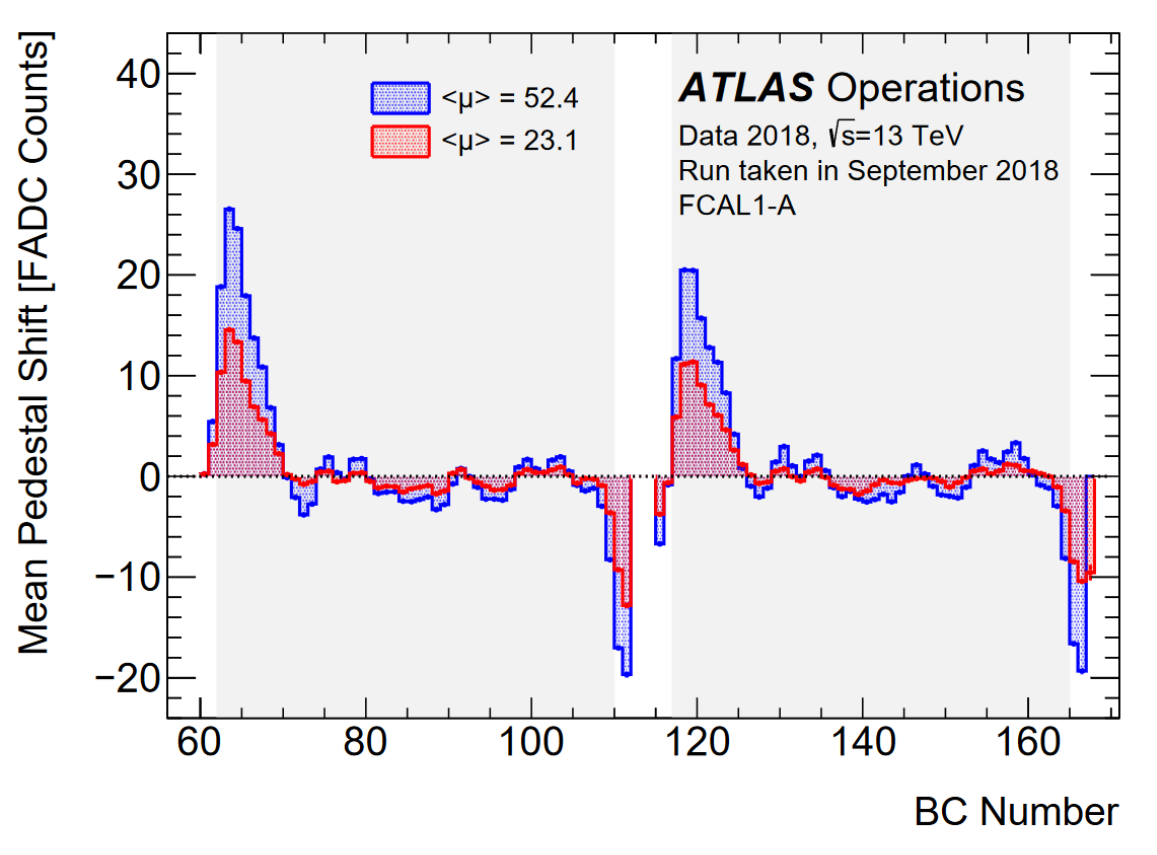
\includegraphics[width=0.6\textwidth]{Chapter6/pedestalCorr.png}
  	\begin{center}
  		\caption{The pedestal correction as a function of bunch crossings for long bunch trains. The shadowed area is within a bunch train\cite{Jongmanns:2661780}.}
  		\label{Fig:pc}            
  	\end{center}
\end{figure}
\begin{figure}[!h]                
	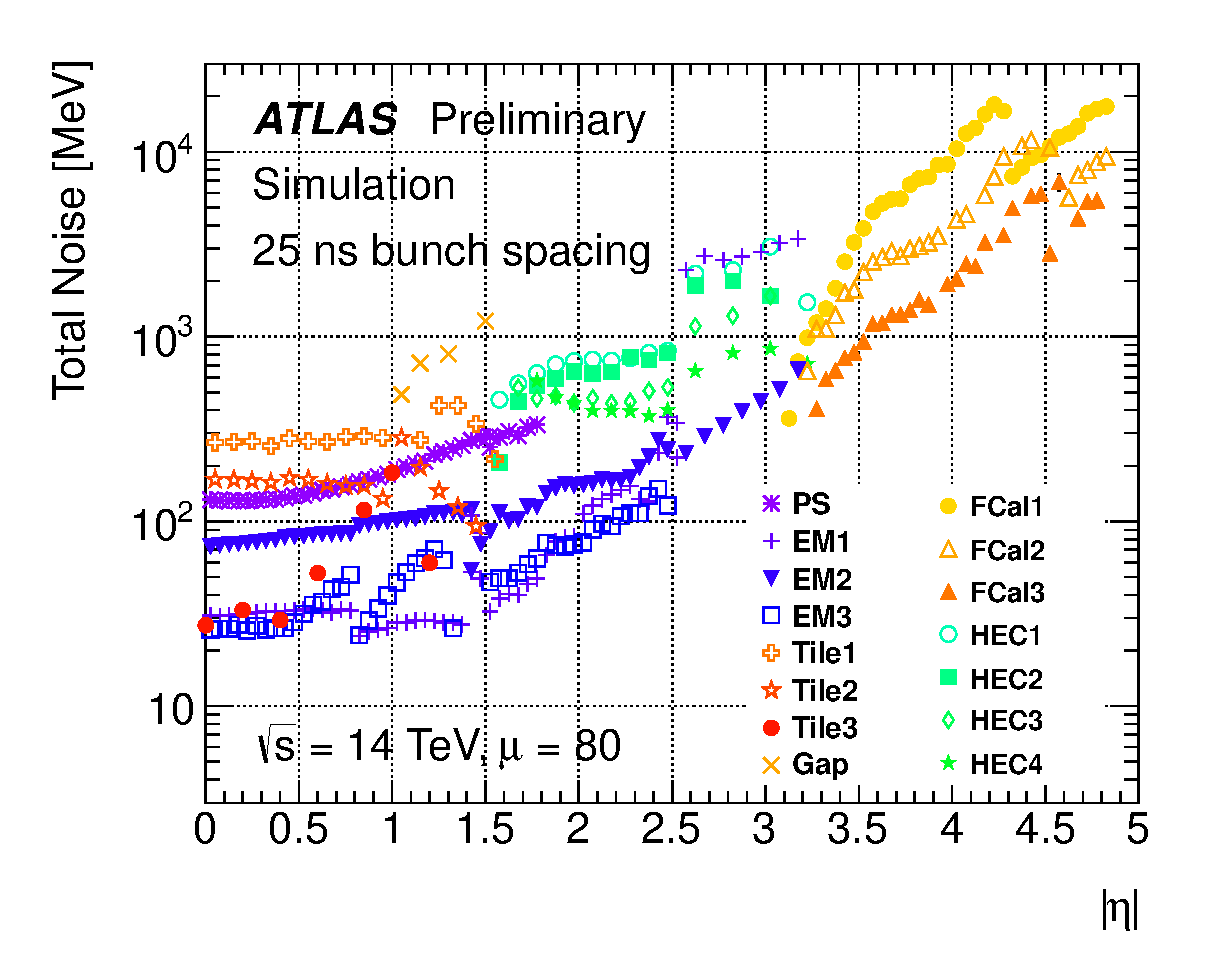
\includegraphics[width=0.6\textwidth]{Chapter6/noise_tot_plot_OFLCOND-MC12-HPS-19-60-25.eps}
	\caption{The average $E_{T}$ of supercell layers as a function of $|\eta|$ with the Run~2 like algorithm with peak finder algorithm\cite{Aleksa:1602230}}
	\label{Fig:sc_noise}            
\end{figure}
\noindent
\\
\\The calibrated supercells are taken as the input for eFex, and they are reconstructed into electrons/photons, and taus with the coverage of $|\eta|$ up to 2.5 (For physics analysis, this is also the $|\eta|$ range for offline electrons due to the coverage of inner detector). It should be noted that in the hardware trigger level, electrons and photons are reconstructed into the same objects for no track information. The reconstruction is performed from seed-finding in the EMB2 layer with the finest granularity and greatest depth. The energy of tTowers behind the ROI are then added into the reconstruction object in EM layers. With the upgraded system, the algorithms could have more flexibility to explore different cluster shapes and also the isolation variables. Further details will be discussed later. 
\\
\\{\bf jFex and jTower}
\\
\\jTowers are in a similar format as the Run~2 trigger towers with the same granularity, $0.1\times0.1$, but it is not uniform in the whole detector. The granularity of each regions in the barrel and endcap regions is summarized in Tab.~\ref{Tab:granularity_jT}.
\begin{table}[h]
	\caption{The jTower granularity in the barrel and endcap regions}
	\renewcommand{\arraystretch}{1.3}
	\centering
	\begin{tabular}{| c | c | c | c | }
		\hline
		\hline
		Index      &    $|\eta|$        &     $\Delta$     & $\Delta\phi$   \\
		\hline
		0          &     0-2.5          & 0.1                          &  0.1                          \\
		\hline
		1          &     2.5-3.1           & 0.2                          &  0.2                         \\
		\hline
		2      &     3.1-3.2       & 0.1                       &  0.2                       \\
		\hline
		\hline
	\end{tabular}
	\label{Tab:granularity_jT}
\end{table}
\noindent
The construction of the jTowers are firstly performed by defining the static windows for the jTowers sizes and locations. Then, those windows are simply matched to the supercells whose energy is summed over to build the $E_{T}$ of jTowers. No additional selection of supercells is applied. However, for the forward region, this construction can't work because of the irregular shape of supercells, and one supercell might overlap with two other supercells in a back layer. In this case, all the supercells are taken as jTowers directly, so the layer information would still be kept. For the input from the tile detector, the tTowers are processed into independent jTowers in the jFex, so there would be two trigger towers at the same location corresponding to EM and hadronic layers. 
\\
\\When the jFex is processing the jTowers, it is performed in eight FPGA modules which receive data from each $\phi$-octant respectively covering the full $\eta$ range ($0<|\eta|<4.9$) from the barrel to forward region, and the jTower data is duplicated to the neighbouring FPGAs\cite{Aad:1602235}. This is to properly reconstruct the physical objects (jets or large tau) at the transition region between FPGAs. The final outputs of the jFex are taus with larger ROI, small-R jets ($R=0.45$), $E^{miss}_{T}$, and the transverse energy scalar sum ($H_{T}$). Different from the Run~2 system, the new system can afford more computing-expensive algorithms for the event-by-event pile-up mitigation. 
\\
\\{\bf gFex and gTower}
\\
\\The gTowers have similar properties as the jTowers, but they are given a even more coarse granularity of $0.2\times0.2$ without the layer information. Furthermore, not like the jTowers constructed from individual supercells in the forward region, the forward layers of supercells are still summed over to construct the jTowers by defining static windows which collect the supercells with their electrodes inside the region. Tab.~\ref{Tab:granularity_gT} is presenting the gTower granularity in the barrel and endcap regions, while the forward region has the $|\eta|$ binning as:
\begin{equation}
|\eta| = \left[3.2, 3.5, 4.0, 4.45, 4.9\right]
\end{equation}
with bins in $\phi$ with $\Delta\phi\sim0.2$
\begin{table}[h]
	\caption{The gTower granularity in the barrel and endcap regions}
	\renewcommand{\arraystretch}{1.3}
	\centering
	\begin{tabular}{| c | c | c | c | }
		\hline
		\hline
		Index      &    $|\eta|$        &     $\Delta$     & $\Delta\phi$   \\
		\hline
		0          &     0-2.5          & 0.2                          &  0.2                          \\
		\hline
		1          &     2.4-2.5           & 0.1                          &  0.2                         \\
		\hline
		2      &     2.5-3.1       & 0.2                      &  0.2                       \\
		\hline 
		3      &     3.1-3.2       & 0.1                      &  0.2                       \\
		\hline
		\hline
	\end{tabular}
	\label{Tab:granularity_gT}
\end{table}
\noindent
\\
\\With the coarse granularity, there would be fewer input channels to the gFex, so it can afford some more complicated algorithms and increase the region of interest, which is one of the motivations to have the gFex in the Run~3. In the Run~2, the JEP can only handle the ROI for a narrow jet ($R\sim 0.45$), and it is too small for a large-R jet which is an important signature for a wide range of physics analyses. The comparison of the Run~2 and Run~2 trigger level jets could be seen in Fig.~\ref{Fig:ZPrimett}, and the new system could extend the jet reconstruction to contain all the energy deposit for the decays of two close-by hadrons. The other advantage of gFex is that it could allow to have more complicated algorithms than the jFex for the pile-up subtraction. 
\begin{figure}[!h]                
	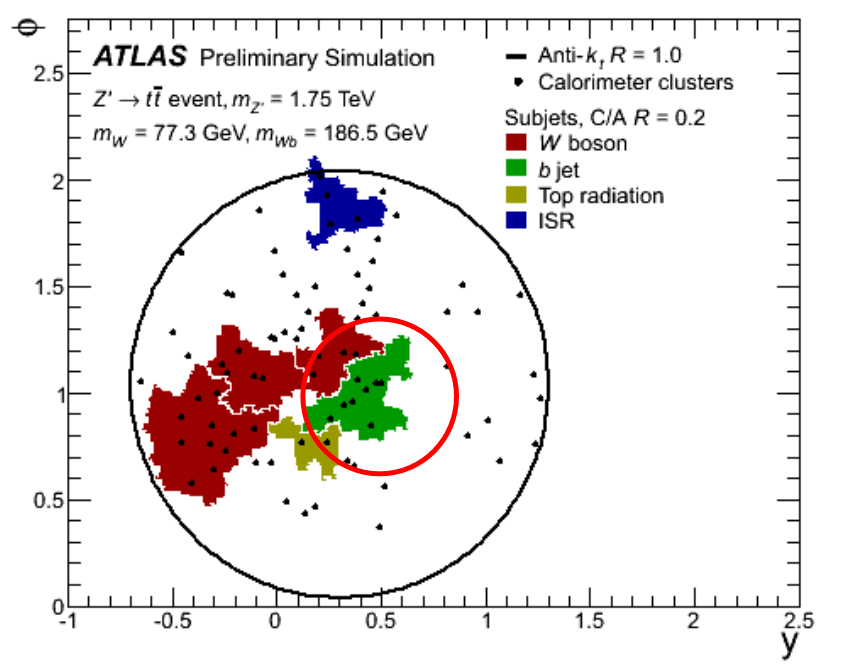
\includegraphics[width=0.75\textwidth]{Chapter6/TrigJetRange.png}
	\begin{center}
		\caption{The comparison of the Run~2 (red circle) and Run~3 (black circle) L1Calo jet ROIs for an HVT $Z'\to t\bar{t}$ event. The Z' boson was given a high mass, so the two top quarks were highly boosted and got close to each other. They would form a large-R jet in the offline reconstruction \cite{Tang:2289434}.  }
		\label{Fig:ZPrimett}            
	\end{center}
\end{figure}
\noindent
\\
\\The processing of gTowers in the gFex is conducted in three FPGAs which correspond to three $\eta$ ranges of full $\phi$ rings:
\begin{itemize}
	\item FPGA $\#A$: $-2.5<\eta<0$
	\item FPGA $\#B$: $0<\eta<2.5$
	\item FPGA $\#C$: $2.5<|\eta|$
\end{itemize}
Due to the bandwidth limit for the communication between these FPGAs, no gTower can be duplicated like as they might be in the jFex. In this case, when reconstruction objects near the border of FPGAs, the gTowers outside the available range are not be considered. In this case, the reconstruction of gFex jets is not yet settled. The outputs from the gFex are the large-R jets and $E^{miss}_{T}$ with another algorithm different from the jFex one.
\section{Simulation Software of the Run~3 ATLAS Calorimeter Trigger}
The general simulation procedure was already introduced in Sec.~\ref{sec:simulation}. However, the Run~3 system is still missing in the simulation chain, so I made the contribution to build up the framework with essential components and integrate it into the ATLAS software, Athena. The final output from the simulation should contain both of the trigger-level and offline objects, so they can be distributed to the physics analysis groups to decide what trigger items should go in the trigger menu for the ATLAS Run~3 operation. 
\\
\\The trigger simulation receives the digitized data from the LAr detector simulation, so the supercells are already defined at the ESD level. The trigger simulation are performed afterwards in the following procedure:
\begin{itemize}
	\item Tower Identification: this process is to define the j/gTower windows in the detector with their locations and granularities through the ATLAS Identifier system.
	\item Supercell $\&$ Tower matching: as the j/gTowers are constructed from the supercells, this is to pair the j/gTowers with the supercells inside the defined windows.
	\item Construction of Towers: this is performed event by event to collect the energy deposits from supercells into the j/gTowers
	\item Event Data Model: this is the format to store the reconstructed objects in the output file including both the hardware level (like tracks, energy cluster, or trigger towers) and physical objects. As new j/gTowers are new objects in the Run~3, an event data model is created to store them.
	\item Physical Object Reconstruction: methods for the phyiscal object reconstruction from the trigger towers. As of July 2019, the baseline electrons from eFex, and small-R jets and $E^{miss}_{T}$ from jFex are already implemented, while the tau reconstruction and gFex objects are still under study. The algorithms for object reconstruction will be discussed in Sec.~\ref{Sec:Trig_obj}. 
	\item Integration: the last step is to integrate the simulation into the ATLAS simulation chain, $reco\_tf$\cite{Stewart:2014ida}, with which the output samples contain all the objects for physics studies with trigger objects. 
\end{itemize}
\noindent
This simulation is under the ATLAS official software, Athena, which is a Gaudi-based system\cite{Mato:2010zz}. All the simulation components are C++ based scripts, and the they are accessible and configurable via python interface (jobOption) under this framework.
\subsection{Tower Identification}
The ATLAS identifier (ID) infrastructure\cite{Schaffer:684167,Arnault:2003pa} is used to define and interpret the hardware readout channels for the offline system\footnote{offline means the system is detached from the detector}. It has two components, the dictionary and ID helper. The dictionary is to categorize the hardware readout channels in a hierarchy structure which decomposes the ATLAS detector into several levels, and the ID helper is to interpret the dictionary to construct the readout channels into offline software via the detector storage\cite{Calafiura:2003gf} which is shared between events. 
\\
\\For the use in the Run~3 L1Calo trigger, the system is deployed to define the jTowers and gTowers, while the supercells are done within the LAr simulation software. However, the identifier system can only be applied on the the readout channels in a regular pattern, so it doesn't extend to the forward region where supercells are in irregular shapes. Therefore, the forward region towers are defined only in the main construction script, and this information doesn't go into the detector storage\cite{Calafiura:2003gf}. 
\\
\\{\bf Dictionary}
\\
\\The definition dictionary is written in the format of xml, which decomposes the detector in the following order:
\\
\\the ATLAS detector $\to$ subdetectors $\to$ detector sides ($+\eta$, $-\eta$) $\to$ region (barrel, endcap) $\to$ sampling layer (EM/Had) $\to$ $\eta$ $\to$ $\phi$
\\
\\Under this structure, each of the readout channel is given an unique hash number with a set of indices representing its hardware location within each level. With the hash numbers, the readout channels could only be recognized by the indices, and the physical meaning like the real $\eta$, or $\phi$, would still need the further interpretation in the script for a proper construction to make the readout channel into an object (j/gTower in this case). The following is a snippet of how the readout channels are defined in the dictionary:
\\
\begin{lstlisting}{listing only}[language=xml]
<field name="JTsampling" > 
  <label name="EM"       value="0" /> 
  <label name="Hadronic" value="1" /> 
</field> 
	
<subregion name="JTower" > 
  <range field="DetZside"
      values="negative_lvl1_side positive_lvl1_side" /> 
  <range field="JTsampling" values="EM Hadronic" /> 
</subregion> 
	
<!-- Up to eta=2.5 --> \\
<region group="Reg\_JTower" name="JTower\_0" 
      eta0="0.0" deta="0.1" phi0="0.0" dphi="0.1"> 
  <reference subregion="JTower" /> 
  <range field="JTregion" value="0" /> 
  <range field="JTeta" minvalue="0" maxvalue="24" />
  <range field="JTphi" minvalue="0" maxvalue="63" 
      wraparound="TRUE" /> 
</region>
	
\end{lstlisting}
\noindent
The first block in the script defines the two layers of the jTowers, EM and Hadronic layers, and the second block is for the two detector sides. Then, the definition for the central region (region index as 0) granularity and the beginning point of $\eta$ and $\phi$ is shown in the third block, and each tower would be given the $\eta$ indices ranged from 0 to 24 and $\phi$ indices ranged from 0 to 63. For the jTowers, there are three regions defined corresponding to the granularities presented in Tab.~\ref{Tab:granularity_jT}, while gTowers are categorized into five regions which is summarized in Tab.~\ref{Tab:granularity_gT}. The system would then loop through the combinations of those indices to build up all the trigger towers within those regions, assign the unique hash numbers for each trigger tower via the ID helper, and register them into the detector storage\cite{Calafiura:2003gf}.
\\
\\{\bf ID Helper}
\\
\\We designed the id helper to interface the dictionary and the user code for the simulation of the ATLAS detector written in the format of C++. For each system, a dedicated helper is customized due to different architectures of the subdetector designs. During the initialization of the identifiers, the helpers would access its corresponding dictionary and assign the hash identifiers for each channel by the set of indices. The identifier is then enumerated and cached for fast conversion. Under this framework, the memory for the cache of Run~2 identifiers is already fixed and filled, and the direct addition of Run~3 identifiers would occupy the memory. In this case, the identifiers would not be properly configured. To add in the new Run~3 trigger tower identifiers, the Run~2 trigger tower caches are expanded by the method in the snippet shown below:
\\
\begin{lstlisting}{listing only}
m_full_region_range = m_dict
                 ->build_multirange(reg_id,"Reg_Lvl1" ,prefix, "region");
m_full_tower_range = m_dict
                 ->build_multirange(reg_id,"Reg_Lvl1" ,prefix, "phi");
m_full_layer_range = m_dict
                 ->build_multirange(reg_id,"Reg_Lvl1" ,prefix);
\end{lstlisting}
\noindent
This function is to make the new jTower and gTower identifiers as the extension of the Run~2 trigger towers, so both the Run~2 and Run~3 trigger tower systems could run in parallel. After the identifiers are cached, the users could then access the tower information via the detector StoreGate (DetStore)\cite{Calafiura:2003gf} in the Athena framework. 

\subsection{j/gTower Matching and Construction}
The tower definition is then taken to build up the tower windows on the calorimeter for which the locations are fixed. The following snippet is to show how the windows are defined in the software:
\\
\begin{lstlisting}{listing only}
float jDEta = m_jTowerId->etaGranularity(rid);
float jDPhi = m_jTowerId->phiGranularity(rid);
int nTowers = (int)(TMath::Pi()/jDPhi)+1;
jDPhi = TMath::Pi()/nTowers;

float jEta = (m_jTowerId->eta(jid)+1-0.5)*jDEta*detSide
                                  +m_jTowerId->eta0(rid)*detSide;
float jPhi = (m_jTowerId->phi(jid)+1-0.5)*jDPhi+m_jTowerId->phi0(rid);
if(jPhi>TMath::Pi()) jPhi = jPhi-2*TMath::Pi(); 
\end{lstlisting}
\noindent
\\Firstly, the granularities are taken from the dictionary by the region with $\Delta\phi$ redefined to ensure the number of $\phi$ segments is an integer. Then, $\eta0$ and $\phi0$ are used to define the starting point of this region with the granularity to evaluate the centre of trigger towers, and the trigger towers are defined with $\eta$, $\phi$, and its granularity. For the forward region, the j/gTower are not defined in the dictionary, so another approach is taken. For the jTowers, a simple scheme is deployed to take the forward supercells as individual towers from $|\eta|=3.1$, while forward gTowers are hard-coded to define the edge and granularity of the towers in the simulation software as the following:
\\
\\
\begin{lstlisting}{listing only}
float fgT_Etas[5] = {3.2, 3.5, 4.0, 4.45,4.9};
int nTowers = 17;
float fgT_dPhi = 2*TMath::Pi()/nTowers;
\end{lstlisting}
\noindent
\\For the supercells, the supercell identifier is used to retrieve the locations of the electrodes, and the following is the snippet for this purpose:
\\
\begin{lstlisting}{listing only}
float scEta = dde->eta_raw();
float scPhi = dde->phi_raw();
if(fabs(scEta)>3.2) continue;
if(fabs(fabs(dde->eta_raw())-1.4)<0.001 && m_scid->region(scid) == 0 
    && m_scid->sampling(scid) == 2){
  if(scEta > 0) scEta += 0.05;
  else          scEta -= 0.05;
}

\end{lstlisting}
\noindent
It could be noted that the $\eta$ and $\phi$ are taken ``raw'', and that means the locations applied in the study are not calibrated for any misalignment in the reality. The last section of the script is showing a special case that the supercells near the transition region between barrel and endcap regions are on the edge of supercells, and the adjustment is to ensure they could be mapped to the trigger towers beginning at $|\eta|=1.4$.
\\
\\After both towers and supercells are defined, a matching is performed by verifying whether the supercells are inside the tower windows. If they are matched, the supercell indices are serialized into a vector as one auxiliary parameter of the towers. Then, the energy of towers is evaluated by simply summing over all the supercells inside the tower window.
\subsection{Event Data Model for j/gTowers}
The ATLAS event data model\cite{Buckley:2015tjh} (EDM) was constructed to store and handle the variables from physical and detector objects. Each type of objects such as electrons, jets, or trigger towers, has one dedicated event data model which is called a container. For the j/gTowers, the Run~2 trigger tower container could not meet all the requirements to store new variables, so a new container was created for them.
\\
\\The ATLAS EDM is based on C++, and the scheme is shown in Fig.~\ref{Fig:edm}. With this infrastructure, the objects are constructed as two components, the object itself, and the object parameters like $E_{T}$ or $\eta$. The object parameters are then taken into the auxiliary store of the object, and the object could access the auxiliary store to obtain the variables. When the objects are built up for an event, they are serialized into a vector (transient data) which are then dumped into the container and aux-container (persistent data) respectively via StoreGate\cite{Calafiura:2003gf} and written out into a ROOT file. The StoreGate feature could then also be used to retrieve the object information from the containers.
\begin{figure}[!h]                
	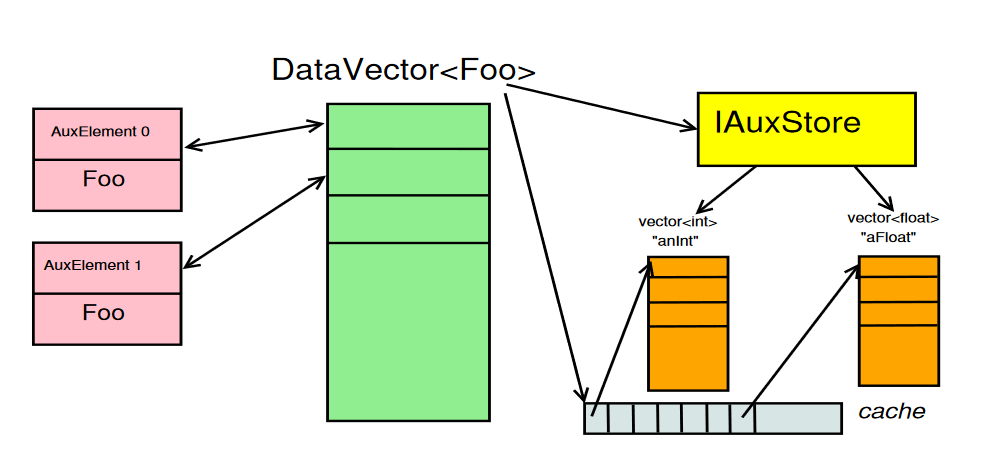
\includegraphics[width=0.75\textwidth]{Chapter6/EDM.png}
	\begin{center}
		\caption{The illustration of the ATLAS EDM scheme for the auxiliary store\cite{Buckley:2015tjh}.}
		\label{Fig:edm}            
	\end{center}
\end{figure}
\noindent
\\The new container design is following the same structure as the Run~2 trigger tower container, and the scheme is skimmed by removing the redundant variables. Those removed variables are used for the LAr detector readout calibration like the bunch crossing index and the information about the pulse peak which are now processed in the supercell construction, and they are irrelevant to the j/gTowers. As the j/gTowers are now constructed from the supercells, the indices of supercells inside the towers are now also added into the container for the potential use of pulse shape inside the towers. 
\subsection{Simulation Chain Integration}
To study the trigger performance for physics analyses, both of trigger-level and offline objects are used to understand the trigger threshold impact on a physics results like the study in Sec.~\ref{Subsec:Trigger_resonance}. Therefore, the new trigger simulation component was integrated into the ATLAS simulation chain to run the tower simulation with the other components have samples containing trigger-level and offline objects.   
\\
\\The simulation is handled by the $reco\_tf$ function built in the Athena framework which is presented in the scheme in Fig.~\ref{Fig:reco_tf}. It is in the form as a python script which calls all the default reconstruction components within the Athena framework using the configurations corresponding to the Athena version (which is called ``release'' in the ATLAS collaboration). The most important feature in the framework is in the middle block where multiple steps of the reconstruction could be executed sequentially by taking the output file from the last step as a new input. This means although the simulation is complicated as shown in Sec.\ref{sec:simulation}, it could still be completed with just a simple command. The other feature of the system is that the completed jobs would send the metadata information such the processed event number and interaction cross-section to the ATLAS Metadata Interface (AMI). The $reco_tf$ script could also be extended to include new reconsturction component by the subcommands, preExec and postExec, and this is used to integrate the Run~3 trigger simulation into the simulation chain. The execution order of components from the $reco_tf$, preExec, and postExec is shown in Fig.~\ref{Fig:exeOrder} where the execute() is to run the default algorithms in $reco_tf$. 
\\
\\The following is the snippet showing how the Run~3 trigger simulation runs with the $reco_tf$ script:
\\
\begin{lstlisting}{listing only}
Reco_tf.py \
--preExec \
  "from TrigT1CaloFexSim.L1SimulationControlFlags 
                   import L1Phase1SimFlags as simflags;\ 
  simflags.CTP.RunCTPEmulation=False; \
  simflags.Calo.QualBitMask=0x40; \
  simflags.Calo.SCellType=\"Pulse\";
  simflags.Calo.ApplySCQual=True" \
--postInclude \
  "default:PyJobTransforms/UseFrontier.py" \
  "TrigT1CaloFexSim/createL1SimulationSequence.py" \
  "LArROD/LArConfigureCablingSCFolder.py" \
--postExec \
 "StreamAOD.ItemList+=["xAOD::JGTowerContainer#JTower","xAOD::JGTowerAuxContainer#JTowerAux."]; \  StreamAOD.ItemList+=["xAOD::JGTowerContainer#GTower","xAOD::JGTowerAuxContainer#GTowerAux."]";
--autoConfiguration="everything" \
\end{lstlisting}
\noindent
The preExec is to set up the Run~3 configuration for the whole simulation chain, and the postInclude here plays the same role as the postExec with the algorithm components inside joboption files (in python format) which is to run the Run~3 trigger simulation. As the new trigger towers are not set as the default output, they are added by the postExec to dump the containers and the corresponding auxiliary containers into the output AOD files. The last subcommand is to set the simulation to run with the default configuration for the detector geometry and database which has the information like the employed high voltage in calorimeter or the threshold to receive the cell energy. Then, the final output would be the proper sample for further study on the trigger performance.
\begin{figure}[!h]                
	\includegraphics[width=0.70\textwidth]{Chapter6/reco_tf.png}
	\begin{center}
		\caption{The illustration of the ATLAS simulation flow run by $reco\_tf$ with the Athena framework\cite{Stewart:2014ida}.}
		\label{Fig:reco_tf}            
	\end{center}
\end{figure}
\begin{figure}[!h]                
	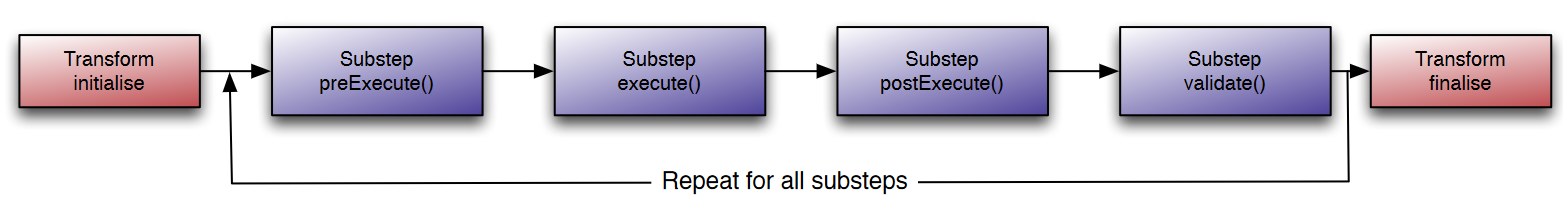
\includegraphics[width=0.85\textwidth]{Chapter6/exeOrder.png}
	\begin{center}
		\caption{The execution order of $reco\_tf$ with its subcommands\cite{Stewart:2014ida}.}
		\label{Fig:exeOrder}            
	\end{center}
\end{figure}
 
\section{Run~3 L1Calo Performance}
\label{Sec:Trig_obj}
The output trigger towers are then taken into the physical object reconstructions. This study is to follow the Run~2-like algorithms to verify the performance of object reconstruction under the new Run~3 system, which will be taken as the baseline reconstruction in the firmware. In the study here, three objects will be discussed, which are electrons, small-R jets, and $E^{miss}_{T}$, and a deeper insight will be given for $E^{miss}_{T}$ reconstruction for which I make a thorough study on the threshold and performance. 
\\
\\The reconstruction of hardware level objects has more constraints than the offline ones. Firstly, the processing of each event must be within the available latency, so a computing-expensive algorithms is not allowed like a machine learning reconstruction with a large-scale structure. Other hardware limit include restriction on communicating links between the readout channels which are rather important for the gFex algorithms, as the three FPGAs don't share the signal connections between each other. Thirdly, the L1Calo objects should still be consistent to the the HLT and offline objects, because the they are taken as the seeds for the HLT reconstruction and required to be matched to offline objects. 
\\
\\To investigate the performance of algorithms, two parameters are studied: trigger rate and signal efficiency of an individual L1 trigger item. The trigger rate is estimated from a minimum bias sample with the luminosity corresponding to the pile-up number as 60 per bunch crossing ($\mu=60$) and $\sqrt{s}=14~TeV$, and it is defined as the following:
\begin{equation}
Rate = 40\times C\times\frac{N^{pass}}{N^{all}}~[MHz]
\end{equation} 
The ``40~MHz'' is corresponding to the collision rate of the LHC multiplied by a factor, C, correcting for the fraction of unfilled bunches and the ratio of events passing the trigger requirement. In the following studies, C was taken as $3/8$ from a run in 2017. Each L1Calo item (the objects with corresponding thresholds) should meet the expected individual Run~3 trigger rate budget in the technical design report which are presented in Tab.~\ref{Tab:trig_rate}. After finding a threshold giving a reasonable trigger rate, the trigger efficiency was studies by the offline turn-on curves (definition could be found in Subsec.~\ref{Subsec:Trigger_resonance}), which should present a sharp turn-on reaching the plateau at a reasonable offline threshold. 
\begin{table}[h]
	\caption{The expected Run~3 trigger rate budget for the L1Calo items (not all of them)}
	\renewcommand{\arraystretch}{1.3}
	\centering
	\begin{tabular}{| c | c | c | c | }
		\hline
		\hline
		Object           &    L1 threshold~[GeV]    &   offline threshold~[GeV] & Rate~[kHz]   \\
		\hline
		electron/photo   &     25                   &   32                      & 14          \\
		\hline
		jet              &     100                 & 200                        &  7        \\
		\hline
		$E^{miss}_{T}$   &     70                  & 200                      &  13                       \\
		\hline
		\hline
	\end{tabular}
	\label{Tab:trig_rate}
\end{table}
\subsection{Electron/photon}
Due to the lack of the track information, the photons and electrons (egamma) are reconstructed from the calorimeter energy deposits into the same object at L1Calo level. With respect to the other signatures, the energy deposit from the egamma  showers is relatively narrow, so the region of interest is defined as a small windonw of the size, $3\times2$, on the $\eta-\phi$ plane (as the green area shown in Fig.~\ref{Fig:ele_iso} corresponding to $0.075\times0.2$ for $\Delta\eta\times\Delta\phi$) with the centre cell as a local maximum inside a three by three window. Its energy is given by the summation of energy over all the sampling layer inside this region of both the LAr and tile detectors. However, the electrons are easily faked by the hadronic objects as discussed in Sec.~\ref{sec:multijet_background}, and a simple cut on energy threshold is not enough to reduce the rate from background easily. In this case, the shower shape of the energy distribution is taken from three variables for a further background reduction:
\begin{itemize}
	\item $R_\eta=1-E_{T}^{3\times2}/E_{T}^{7\times3}$: this variable is defined as as the ratio of energy in green over yellow area in Fig.~\ref{Fig:ele_iso} to ensure the egamma is well-isolated. 
	\item $R_{had} = E^{Had}_{T}/E^{tot}_{T}$: this is the hadronic energy ratio defined in the blue framed region in Fig.~\ref{Fig:ele_iso}, and it helps to reduce the contamination from the hadronic objects, as they would deposit more energy in the hadronic layers.
	\item $w_{tot}=\sqrt{\sum_i E^{SC_i}_{T}\times(\eta^{SC_i}-\eta^{SC_{max}})^2/\sum E^{SC_i}_{T}}$: this is to defined the shower distribution within the red framed region in Fig.~\ref{Fig:ele_iso}. 
\end{itemize}
The final cuts on the three variables are employed with the energy threshold of 20~GeV for the same rate for Run~2 egamma trigger:
\begin{itemize}
	\item $R_\eta<0.12$
	\item $R_{had}<0.16$
	\item $w_{tot}<0.02$
\end{itemize}

\begin{figure}[!h]                
	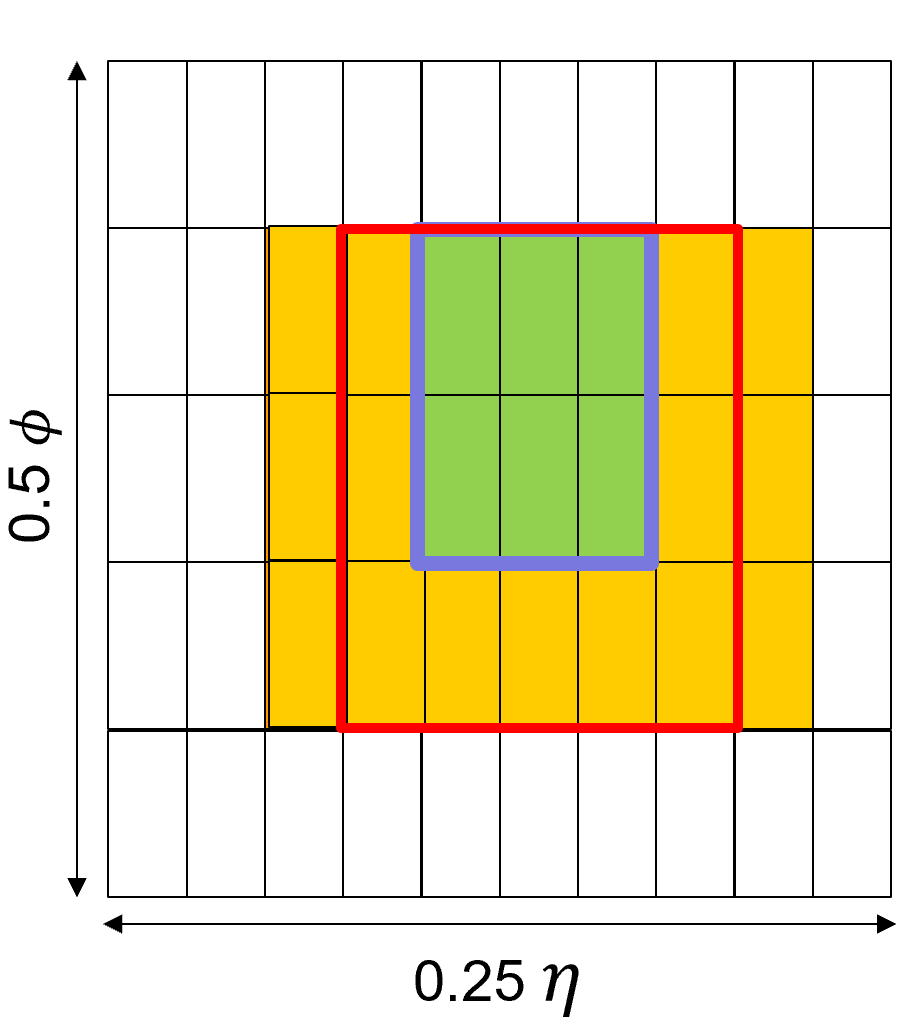
\includegraphics[width=0.4\textwidth]{Chapter6/ele_iso.png}
	\begin{center}
		\caption{The diagram to illustrate the electron/photon ROI with the areas for the isolation definition.}
		\label{Fig:ele_iso}            
	\end{center}
\end{figure}
\noindent
A sample of $Z\to ee$ simulated by Sherpa generator is taken To verify the signal efficiency. The results are presented in Fig.~\ref{Fig:ele_perf}. The turn-on curves as a function of the leading truth electron $E_T$ with an event-veto of truth electrons in the transition region of $1.37<|\eta|<1.52$ are made from two L1Calo electron $E_{T}$ cuts: 20~$GeV$ giving the rate of $\sim30~kHz$ (the Run~2 single electron trigger rate), and 28~$GeV$ giving the rate of $\sim10~kHz$ (the expected rate in the TDR). With the same rate as Run~2 electron trigger, the turn-on curves has shown a sharper turn-on which can reach the plateau at 25~GeV which is 7~GeV lower than the Run~2 offline threshold. For the turn-on curve with the cut on 28~GeV, it reaches the plateau at similar $E_{T}$ as Run~2, but it has much lower rate. Both of them has shown the improvement with respect to the Run~2 electron trigger in terms of either trigger rate or the offline threshold, and it has achieved the performance as the TDR expected. The other study in the trigger efficiency is to verify the $|\eta|$ dependence which is also shown in Fig.~\ref{Fig:ele_perf} with the L1 electron $E_{T}$ cut at 28~GeV. The result has shown that the electron trigger efficiency has low dependence on $\eta$ except for the ones in the transition region, and the trigger has almost $100\%$ for electrons with $E_{T}>30~GeV$.
\begin{figure}[!h]                
	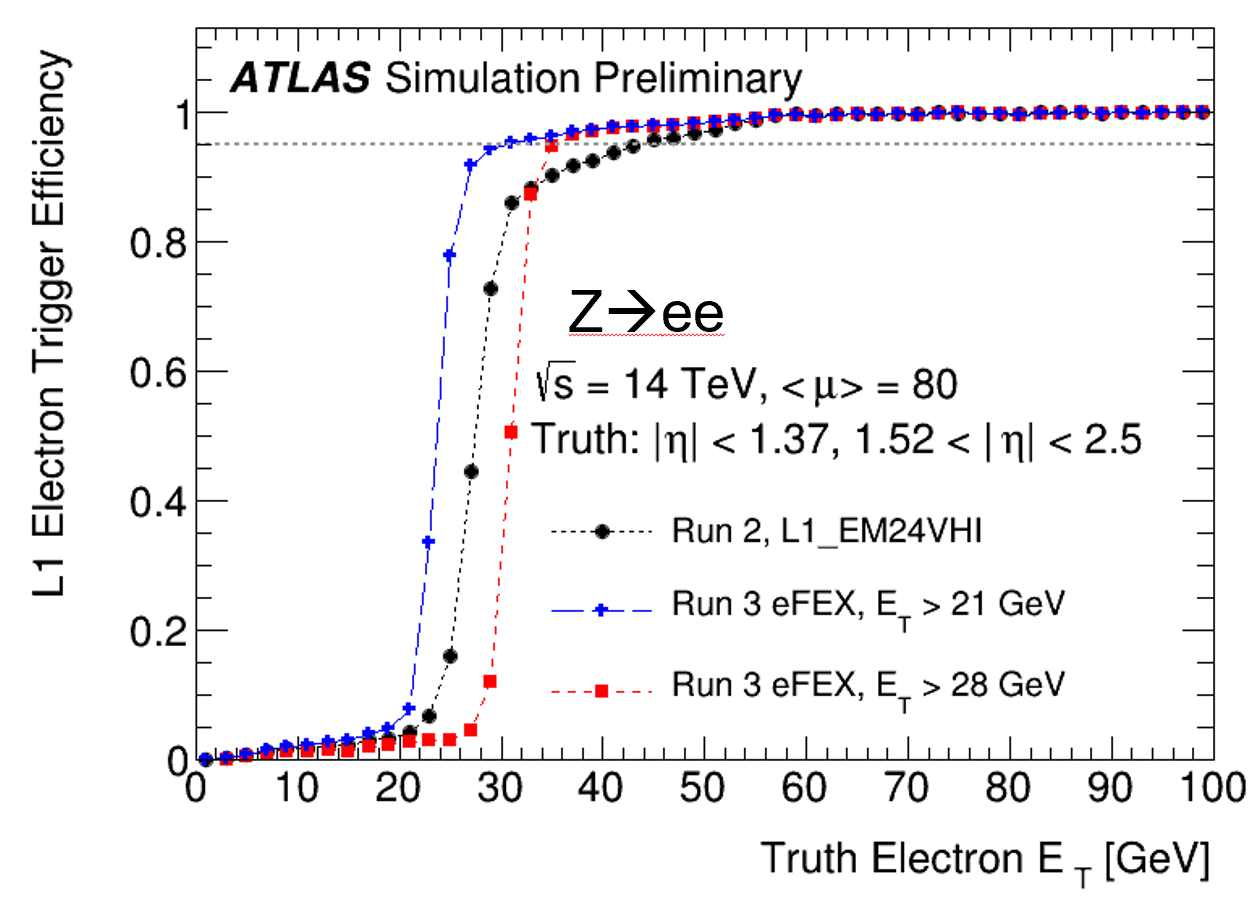
\includegraphics[width=0.45\textwidth]{Chapter6/ele_turnon.png}
	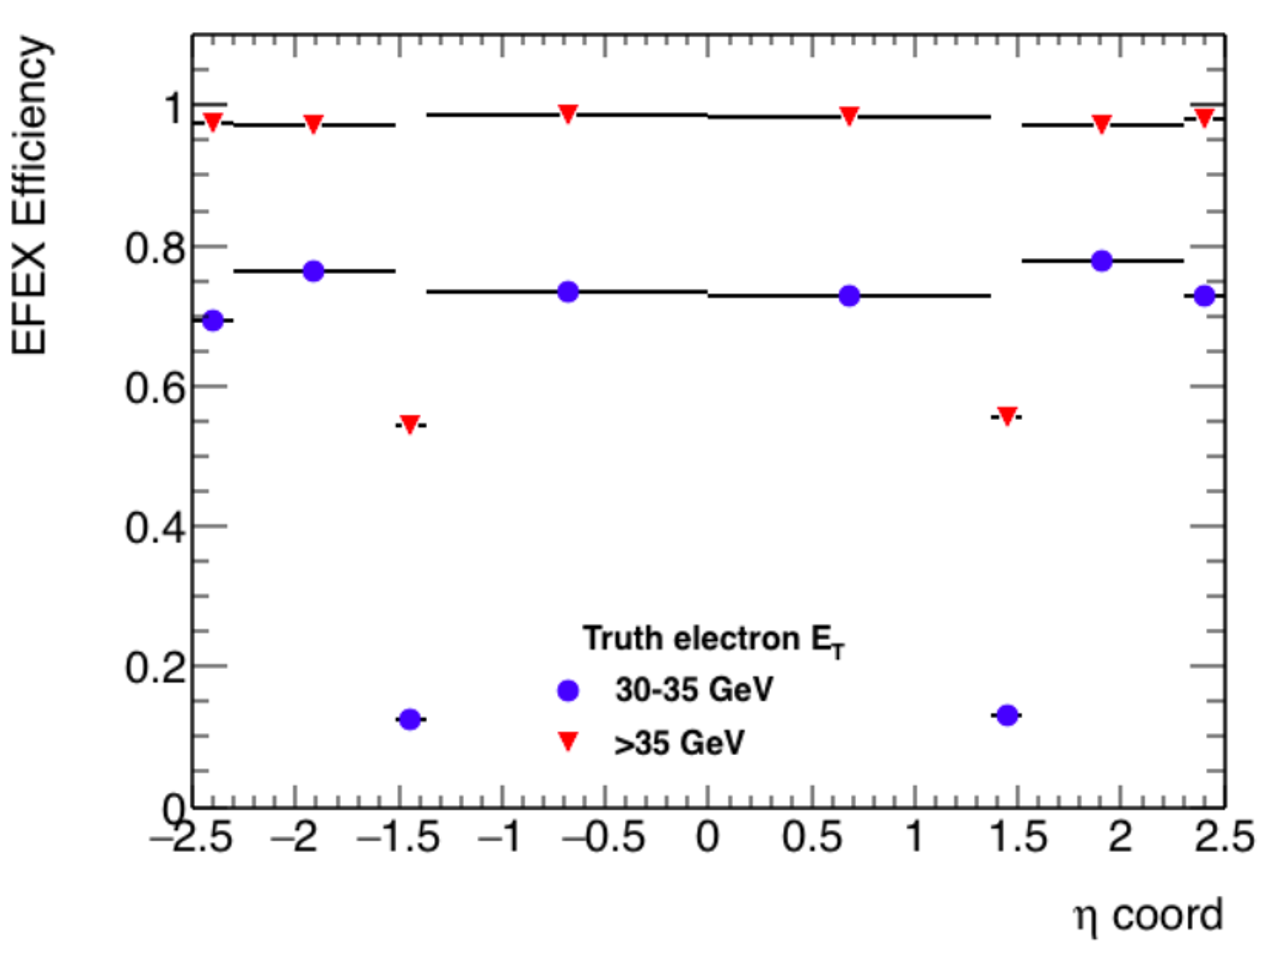
\includegraphics[width=0.45\textwidth]{Chapter6/ele_eta.png}
	\begin{center}
		\caption{The signal efficiency as a function of truth electron $E_{T}$ (left) and $\eta$ (right)}
		\label{Fig:ele_perf}            
	\end{center}
\end{figure}
\subsection{Small-R Jets}
The small-R jets are reconstructed from a sliding window algorithm (SLW). Firstly,  the jet seed finding was performed by a $3\times3$ window ($0.3\times0.3$) which went through the jTowers in the LAr detector. The seed is then built if the centre tower is a local maximum, and the energy sum within the window is above $4~GeV$ and also higher than the surrounding region. Then, the jets is constructed as the region of interest defined as $R=0.45$ from the central tower with the energy summed over both LAr and tile detector sampling layers. It should be noted that the L1Calo jets has a different radius from the offline and HLT ones which have the radius of $R=0.4$, because the number of included towers should be an integer with the centre in a chosen tower. The construction steps are presented in Fig.~\ref{Fig:jet_reco} which is also showing another potential algorithm for which the jets are reconstructed from a $9\times9$ square region of interest. 
\begin{figure}[!h]                
	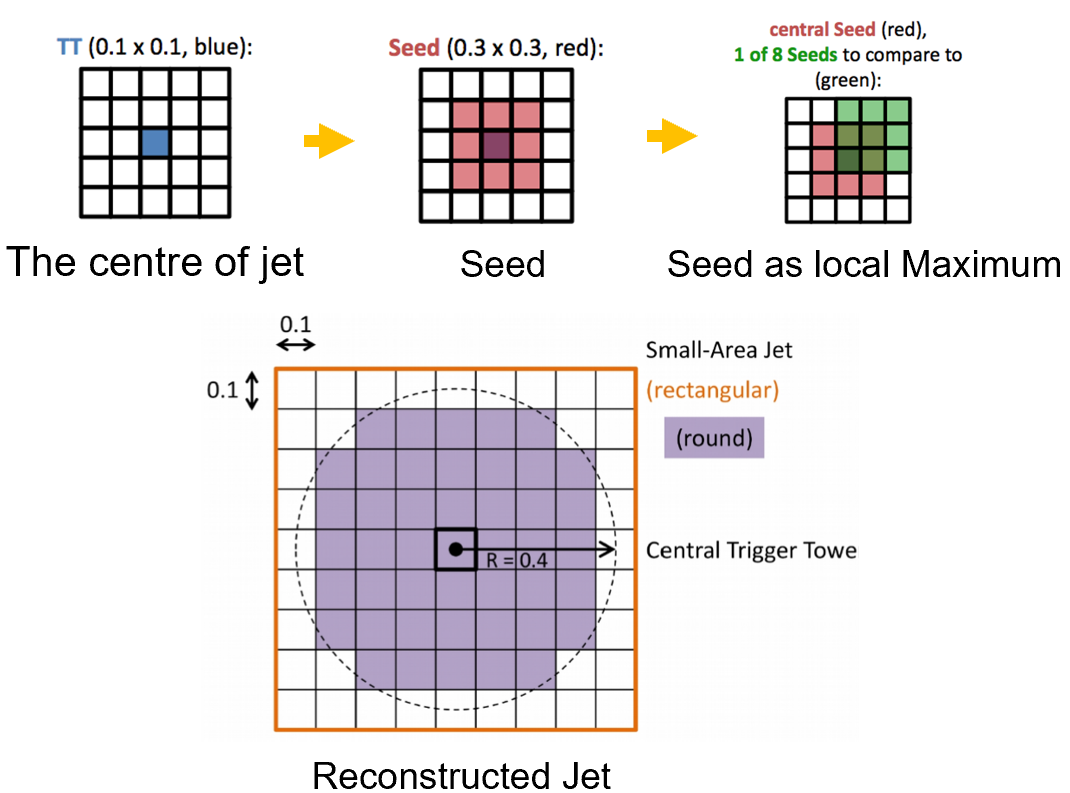
\includegraphics[width=0.8\textwidth]{Chapter6/jet_reco.png}
	\begin{center}
		\caption{The illustration of how the L1Calo jets are reconstructed.}
		\label{Fig:jet_reco}            
	\end{center}
\end{figure}
\noindent
\\
\\For the jet triggers, two L1Calo items are proposed, a single jet trigger and a three-jet trigger. Both of the two triggers are studied with a signal sample of $ZH\to\nu\nu bb$ simulated by Sherpa under the collision environment of $\mu=60$. Although the sample has only two jets from the physical process, the third jet might still be added by the pile-up simulation, so it can also be used for the three-jet trigger study. The performance of these two triggers could be seen in Fig.~\ref{Fig:jet_perf} with turn-ons as a function of the offline first (for the single-jet trigger) and third (for the three-jet trigger) leading jet $E_{T}$. The performance of Run~3 L1 jets is compared to Run~2 L1 jets and anti-$k_{T}$ jets which take jTowers as input entities, and the thresholds are all set giving the same trigger rate. For the Run~3 single jet trigger, the threshold was set at 97~GeV, and it has the same performance as the jets reconstructed from the other two algorithms as what we expect from the TDR (7~kHz). For the three jet trigger, the two Run~3 algorithms has shown better performance than Run~2 jets, as both of them achieve higher efficiency in the turn-on plateau region than Run~2 L1 jets. This is benefited from the improved granularity which provides a better distinguishing power for jet finding within a high pile-up environment.  
\begin{figure}[!h]                
	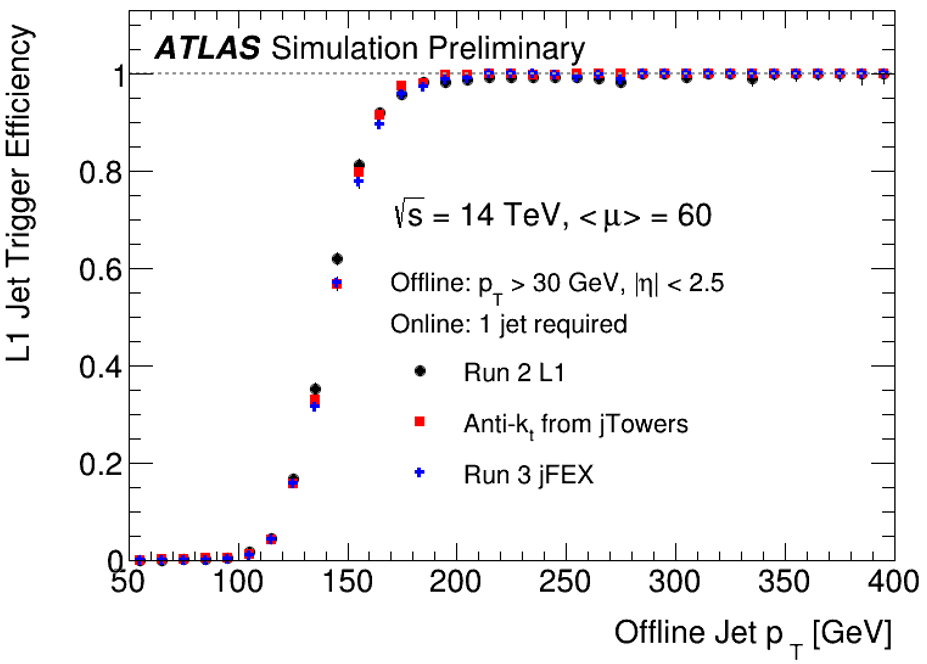
\includegraphics[width=0.48\textwidth]{Chapter6/perf_1jet.png}
	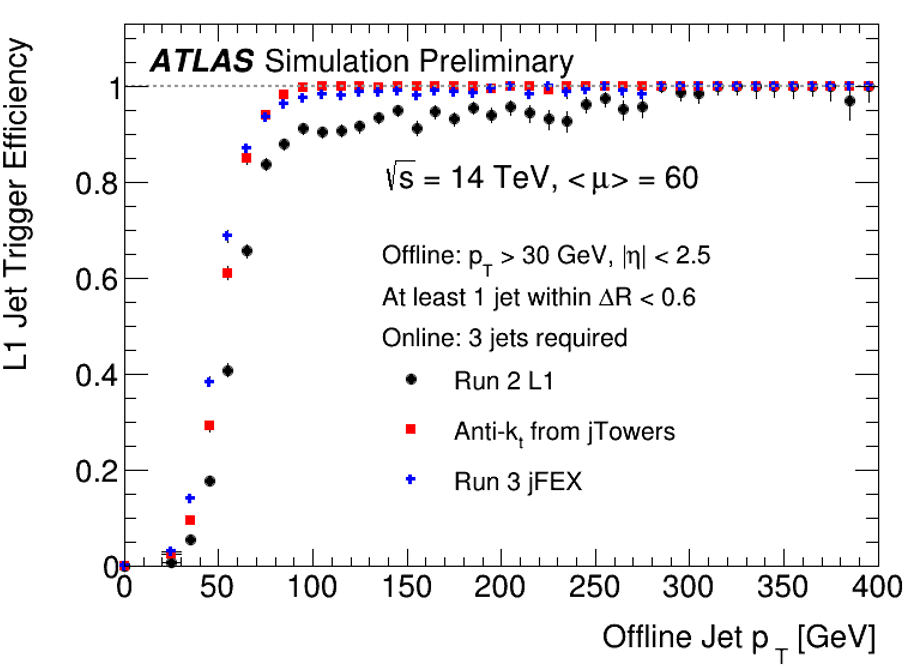
\includegraphics[width=0.48\textwidth]{Chapter6/perf_3jets.png}
	\begin{center}
		\caption{The trigger performance for single-jet (left) and three-jet (right) triggers as turn-on curves as functions of offline jet $E_{T}$}
		\label{Fig:jet_perf}            
	\end{center}
\end{figure}
\subsection{Missing Transverse Energy}
The missing transverse energy, $E^{miss}_{T}$, is constructed as the vector sum of jTowers in the jFex, and the same algorithm proposed here will also be potentially implemented with gTowers which will need further optimization. However, most of the energy deposits in the calorimeter are from the pile-up events or electronic noise, so a proper selection on the towers is essential. With broadly ranged granularities, a constant threshold is not appropriate to handle all the jTowers, so a tower-dependent threshold scheme is applied. For this purpose, the minimum bias sample is used to understand the noise behaviour in the jTowers. The first step is to get the $E_{T}$ histograms for each jTower and take the root mean square (RMS, $1\sigma$) from this histograms, which will be set as the unit of thresholds on jTower selection. Then, the optimization is performed by finding the working point which gives the highest signal efficiency (with the same signal sample for jet trigger study) with the trigger rate at $5~kHz$ as the Run~2 $E^{miss}_{T}$ trigger. The working point scan is performed on a three-dimension phase space constructed by the thresholds on LAr (EM) and tile (Hadronic) sampling layers with one more dimension which levels up the thresholds in the forward region. Fig.~\ref{Fig:thresold_scan_1} is presenting the result of signal efficiency at the trigger rate of $5~kHz$ with the scanning step of $0.5\sigma$ for both LAr and tile towers, while the threshold on the forward region is $0.5\sigma$ higher than the LAr threshold. After this process, the scheme of thresholds shown in Tab.~\ref{Tab:cuts_met} is chosen to reconstruct the jFex $E^{miss}_{T}$.
\begin{table}[h]
	\caption{jTower thresholds for the $E^{miss}_{T}$ reconstruction}
	\renewcommand{\arraystretch}{1.3}
	\centering
	\begin{tabular}{| c | c | c | c | c |  }
		\hline
		\hline
		LAr             &    Tile         &     Forward       & Efficiency & Threshold   \\
		\hline
		$>5\sigma$       &    $>5.5\sigma$  &     $>5.5\sigma$   &  $21.62\%$  &  57~GeV  \\
		\hline
	\end{tabular}
	\label{Tab:cuts_met}
\end{table}
\begin{figure}[!h]                
	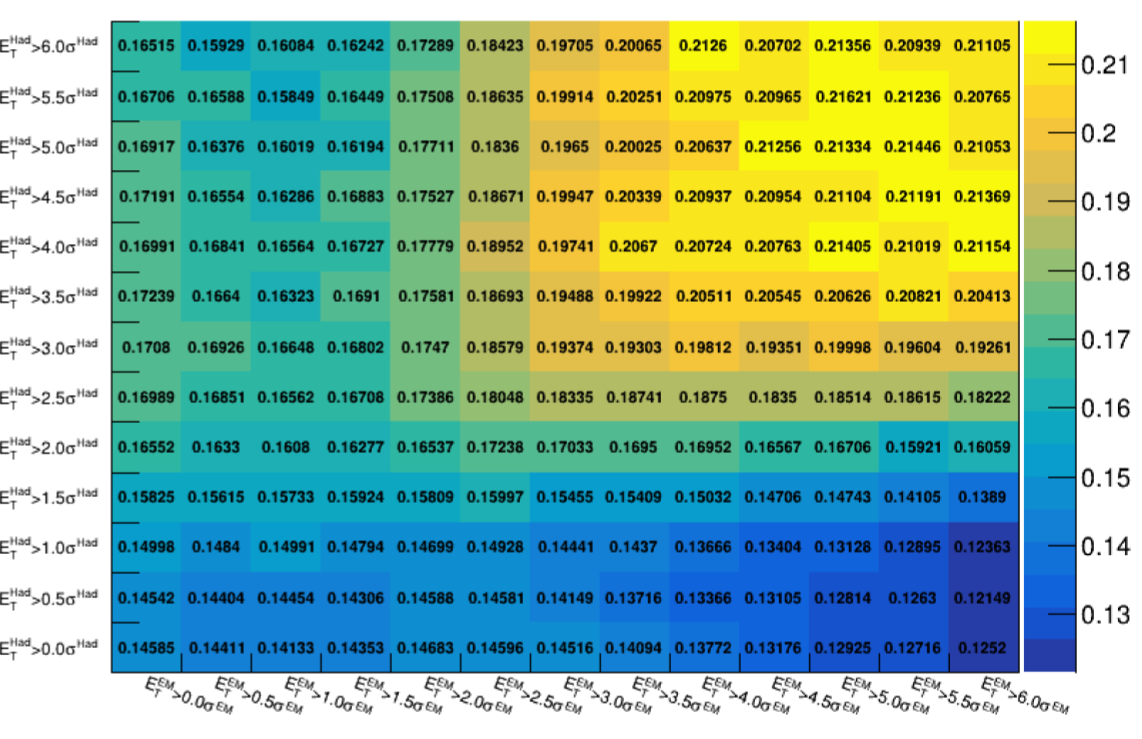
\includegraphics[width=0.48\textwidth]{Chapter6/efficiency_5kHz_cfg1.png}
		\begin{center}
		\caption{The signal efficiency with the trigger rate at $5~kHz$ as a function of thresholds on the LAr (x-axis) and tile (y-axis) $E_{T}$ which are in the unit of $\sigma$. The forward region has the threshold for $0.5\sigma$ higher than the LAr tower threshold.}
		\label{Fig:thresold_scan_1}            
	\end{center}
\end{figure}
\noindent
\\To verify the performance for the physics analysis, the $ZH\to\nu\nu bb$ sample is still used. The first verification is for the energy and spatial resolutions with respect to the truth $E^{miss}_{T}$ which are defined as:
\begin{equation}
Res_{E_{T}} = \frac{E^{jFex}_{T}-E^{truth}_{T}}{E^{truth}_{T}} \\
Res_{\phi} = \Delta\phi(E^{jFex}_{T}, E^{truth}_{T})
\end{equation}
The results could be seen Fig.~\ref{Fig:res_met} with the other thresholds which also give high efficiency with trigger rate at $5~kHz$, and they are showing great agreement to the Run~2 L1Calo $E^{miss}_{T}$. However, when making the trigger rate comparison to data, a significant inconsistency was found as shown in Fig.~\ref{Fig:rate_datamc}. For this case, the Run~2 simulated L1 $E^{miss}_{T}$ cannot be used for a proper comparison due to some unknown modelling issue, and, instead, a dataset collected in 2017 with an offline selection of $Z\to\mu\mu$ is used, as muons are invisible for the L1Calo system and make the contribution to L1 $E^{miss}_{T}$. The result is shown in Fig.~\ref{Fig:perf_met}, and a great agreement is observed because of the similar algorithm. This is now already taken as the baseline jFex $E^{miss}_{T}$, while the other pile-up dependent algorithms are still under investigation for both jFex and gFex. 
\begin{figure}[!h]                
	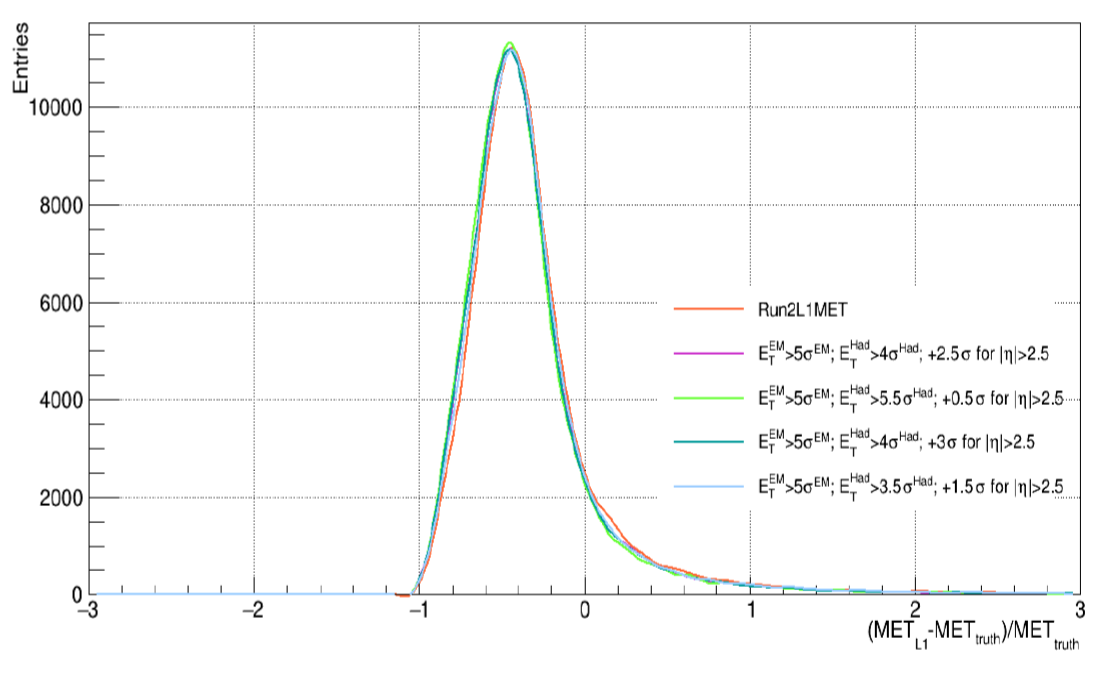
\includegraphics[width=0.48\textwidth]{Chapter6/res_et.png}
	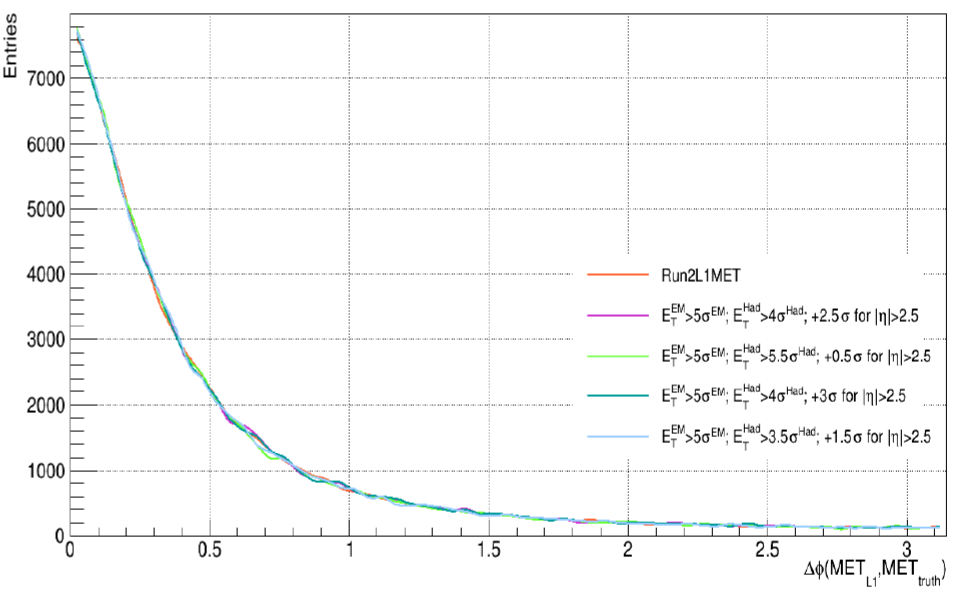
\includegraphics[width=0.48\textwidth]{Chapter6/res_phi.png}
	\begin{center}
		\caption{The energy (left) and spatial resolution of the reconstructed jFex $E^{miss}_{T}$ in comparison to the simulated Run~2 L1Calo $E^{miss}_{T}$}
		\label{Fig:res_met}            
	\end{center}
\end{figure}
\begin{figure}[!h]                
	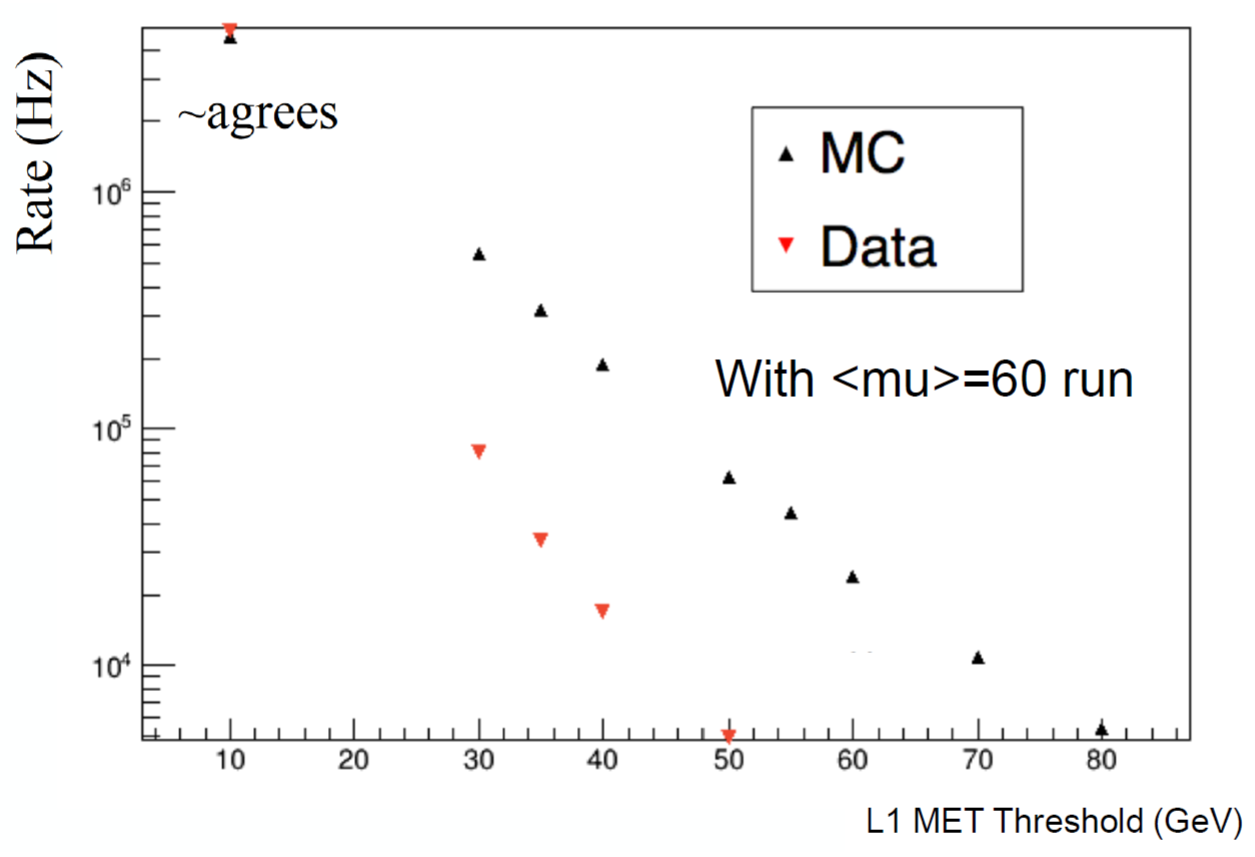
\includegraphics[width=0.45\textwidth]{Chapter6/rate_datamc.png}
	\begin{center}
		\caption{The rate comparison of data and simulated Run~2 L1Calo $E^{miss}_{T}$}
		\label{Fig:rate_datamc}            
	\end{center}
\end{figure}
\begin{figure}[!h]                
	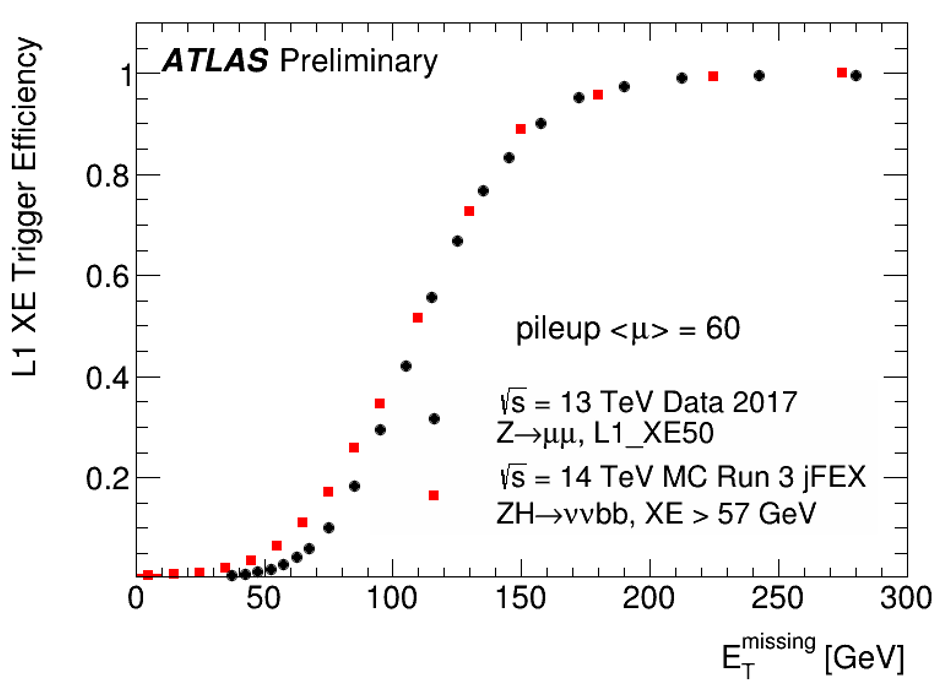
\includegraphics[width=0.57\textwidth]{Chapter6/perf_met.png}
	\begin{center}
		\caption{The efficiency turn-on curves as a function of truth $E^{miss}_{T}$ for data and simulated jFex L1Calo $E^{miss}_{T}$}
		\label{Fig:perf_met}            
	\end{center}
\end{figure}
\section{Summary}
The Run~3 L1Calo upgrade plays an important role for the imminent LHC operation to provide a better background suppression and similar signal efficiency with respect to Run~2 under the environment of abundant pile-ups. The new hardware provides a better granularity and a longer latency for the object reconstruction, and it also grants the flexibility to capture some exotic signatures like the long-lived particles. To make the best use of the new hardware calorimeter trigger system, I have constructed the simulation software with the new trigger towers and integrated into the ATLAS software, Athena. The preliminary studies with my proposed $E^{miss}_{T}$ trigger algorithm have shown promising results, and the samples with the new L1Calo physical objects are also under production in preparation for the Run~3 L1 trigger menu. 